\section{Durchführung}
\label{sec:durchführung}

    Für die Messung der Compton-Wellenlänge ist eine Apparatur gegeben,
    welche eine Röntgenröhre, ein LiF-Kristall und ein Geiger-Müller-Zählrohr enthält.
    Der LiF-Kristall kann durch einen Plexiglasstreuer ausgetauscht werden;
    außerdem können zwischen den einzelnen Bestandteilen Absorber eingebaut werden.\\
    Die Apparatur ist in \autoref{fig:aufbau_röntgen} gezeigt.
    \begin{figure}[H]
        \centering
        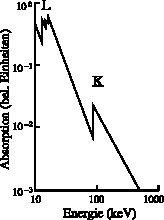
\includegraphics[width=\textwidth]{content/img/Abb_2.pdf}
        \caption{Apparatur zur Erzeugung und Messung von Röntgenstrahlung. \cite{versuchsanleitung}}
        \label{fig:aufbau_röntgen}
    \end{figure}
    Mithilfe der in der Abbildung benannten Bedienelemente können die Röntgenröhre
    sowie die Winkeleinstellung von Kristall und Geiger-Müller-Zählrohr
    manuell bedient werden.

    Die Messung setzt sich aus zwei Teilen zusammen.
    Für alle Messungen werden eine Beschleunigungsspannung von $\SI{35}{\kilo\volt}$
    sowie ein Emissionsstrom von $\SI{1}{\milli\ampere}$ eingestellt.


\subsection{Das Emissionsspektrum der Röntgenröhre}

    Zuerst soll mithilfe des Rechners das Emissionsspektrum der $\ce{Cu}$-Röntgenröhre bestimmt werden.
    Dazu wird das Programm \texttt{measure} ausgewählt,
    in dem unter dem Punkt \texttt{Messgeräte} die Röntgenröhre gesteuert werden kann.\\
    Anschließend werden eine $\SI{2}{\milli\meter}$-Blende und der LiF-Kristall in die Apparatur eingebaut.
    Nun wird zur Messung des Spektrums der Winkel des LiF-Kristalls in Schritten von $\symup{\Delta}\alpha = \SI{0.1}{\degree}$ erhöht mit einer Integrationszeit von $t = \SI{10}{\second}$.


\clearpage
\subsection{Experimentelle Bestimmung der Compton-Wellenlänge}

    Nun soll die Transmission $T(\lambda)$ eines Aluminium-Absorbers untersucht werden.
    Dazu wird der Absorber vor der Blende befestigt.
    In einem Intervall von $\alpha = [\SI{7}{\degree}, \SI{10}{\degree}]$ wird in Schritten von $\symup{\Delta}\alpha = \SI{0.1}{\degree}$ mit $t = \SI{200}{\second}$ nun die Zählrate gemessen.
    Dabei wird einmal die Zählrate ohne Absorber $N_0(\alpha)$
    und einmal mit Absorber $N_\text{Al}(\alpha)$ gemessen.

    Die Totzeit des Geiger-Müller-Zählrohrs $\tau = \SI{90}{\micro\second}$
    erfordert für entsprechend große Zählraten eine Korrektur gemäß der Gleichung
    \begin{equation}
        I = \frac{N}{1 - \tau N} \ .
        \label{eqn:totzeitkorrektur}
    \end{equation}
    \\
    Die nächsten Messungen werden ohne das Rechnerprogramm durchgeführt.
    Dazu wird das Röntgengerät auf \texttt{Manuell} umgeschaltet und das RS232-Kabel entfernt.\\
    \\
    Statt des LiF-Kristalls wird nun ein Plexiglasstreuer in die Apparatur aus \autoref{fig:aufbau_röntgen} eingebaut,
    sowie eine $\SI{5}{\milli\meter}$-Blende.
    Es ist der folgende Aufbau im Inneren der Apparatur gegeben.

    \begin{figure}[H]
        \centering
        \begin{subfigure}{0.4\textwidth}
            \centering
            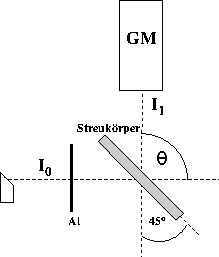
\includegraphics[width=0.65\textwidth]{content/img/Abb_3a.pdf}
            \caption{Messung 1. \cite{versuchsanleitung}}
            \label{fig:aufbau_transmission_a}
        \end{subfigure}
        \begin{subfigure}{0.4\textwidth}
            \centering
            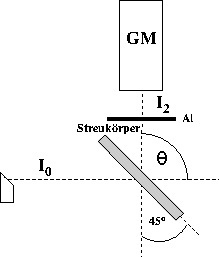
\includegraphics[width=0.65\textwidth]{content/img/Abb_3b.pdf}
            \caption{Messung 2. \cite{versuchsanleitung}}
            \label{fig:aufbau_transmission_b}
        \end{subfigure}
        \caption{Schematische Darstellung der unterschiedlichen Positionierungen des \ce{Al}-Absorbers.}
    \end{figure}

    Mithilfe der \autoref{fig:aufbau_transmission_a} wird nun die Transmission $T_1 = \sfrac{I_1}{I_0}$ der ungestreuten Wellenlänge $\lambda_1$ gemessen,
    indem der Plexiglasstreuer in einem Winkel von $\SI{45}{\degree}$ ausgerichtet wird,
    und das Geiger-Müller-Zählrohr in einem Winkel von $\SI{90}{\degree}$ zur Röntgenröhre.
    Nun wird die Intensität $I_0$ ohne den Absorber in einer Zeit von $t = \SI{300}{\second}$ gemessen,
    sowie die Intensität $I_1$ mit dem Absorber,
    welcher zwischen Röntgenröhre und Plexiglasstreuer eingebaut wird.\\
    Für die gestreute Wellenlänge $\lambda_2$ wird die Transmission $T_2 = \sfrac{I_2}{I_0}$ bestimmt.
    Die Intensität $I_2$ wird gemessen,
    indem der Aluminium-Absorber nach \autoref{fig:aufbau_transmission_b}
    zwischen Plexiglasstreuer und Geiger-Müller-Zählrohr angebracht wird.\\
    Aus der Verschiebung der Wellenlänge $\symup{\Delta}\lambda$ kann nun
    nach \eqref{eqn:wellenlängendifferenz} und \eqref{eqn:verschiebung_winkelabhängig}
    aus \autoref{sec:compton_effekt} die Compton-Wellenlänge $\lambda_\text{c}$ bestimmt werden.
